%----------------------------------------------------------------
%
%  File    :  thesis.tex
%
%  Authors :  David Lechner, FH Campus Wien, Austria
%
%  Created :  10 Oct 2019
%
%  Changed :  10 Oct 2019
%
%----------------------------------------------------------------


% --- General Setup ---------------------------------------------
% !TEX encoding = IsoLatin2
\documentclass[11pt,a4paper,oneside]{scrbook}
\usepackage[T1]{fontenc}
\usepackage[utf8]{inputenc}

\usepackage[ngerman]{babel}

% for nicer PDF rendering. Alternatively, when using MikTeX,
% you could also manually install the cm-super package
\usepackage{lmodern}

\usepackage[T1]{fontenc}

% want Arial? uncomment next two lines...
%\usepackage{uarial}
%\renewcommand{\familydefault}{\sfdefault}

\usepackage[bf,sf]{subfigure}
\renewcommand{\subfigtopskip}{0mm}
\renewcommand{\subfigcapmargin}{0mm}

\usepackage{url}

\usepackage{latexsym}

\usepackage{geometry} % define pagesize in more detail

\usepackage{fancyhdr} % nicer headers and footers

\usepackage{colortbl} % define colored backgrounds for tables

\usepackage{makecell}

\usepackage{multirow}

\usepackage{courier} %for listings
\usepackage{listings} % nicer code formatting
\lstset{basicstyle=\ttfamily,breaklines=true}

  \usepackage[pdftex]{graphicx}
  \DeclareGraphicsExtensions{.pdf,.jpg,.png}
  \pdfcompresslevel=9
  \pdfpageheight=297mm
  \pdfpagewidth=210mm
  \usepackage[         % hyperref should be last package loaded
    pdftex,
    bookmarks,
    bookmarksnumbered,
    linktocpage,
    pagebackref,
    pdfview={Fit},
    pdfstartview={Fit},
    pdfpagemode=UseOutlines,                 % open bookmarks in Acrobat
  ]{hyperref}
  \usepackage{bookmark}

\geometry{a4paper,left=30mm,right=25mm, top=30mm, bottom=30mm}

\setlength{\parskip}{3pt plus 1pt minus 0pt}       % vert. space before a paragraph

\setcounter{tocdepth}{1}        % lowest section level entered in ToC
\setcounter{secnumdepth}{2}     % lowest section level still numbered


% --- Start of Document ----------------------------------------


\begin{document}

\frontmatter
\normalsize
\pagestyle{empty}            % for title pages

%----------------------------------------------------------------
%
%  File    :  title.tex
%
%  Authors :  David Lechner, FH Campus Wien, Austria
% 
%  Created :  10 Oct 2019
% 
%  Changed :  10 Oct 2019
% 
%----------------------------------------------------------------


% --- Main Title Page ------------------------------------------------
\begin{picture}(50,50)
\put(-70,40){\hbox{
\includegraphics{images/FH_Campus_Wien_Logo_Druck_40_mm.png}}}
\end{picture}

\vspace*{-5.8cm}

\begin{center}

\vspace{4.9cm}

\hspace*{-1.0cm} {\LARGE \textbf{Fahreridentifikation mittels Machine-Learning\\}}
\vspace{0.2cm}

\vspace{1cm}

\hspace*{-1.0cm} {\LARGE \textbf{Driver identification using Machine-Learning\\}}
\vspace{0.2cm}

\vspace{2.7cm}

\hspace*{-1.0cm} {\LARGE \textbf{Masterarbeit\\}}

\vspace{0.65cm}

\hspace*{-1.0cm} Zur Erlangung des akademischen Grades \\

\vspace{0.65cm}

\hspace*{-1.0cm} \textbf{Master of Science in Engineering\\}

\vspace{0.65cm}

\hspace*{-1.0cm} der Fachhochschule Campus Wien \\
\vspace{0.2cm}
\hspace*{-1.0cm} Masterstudiengang: ITS-20 \\

\vspace{1.6cm}

\hspace*{-1.0cm} \textbf{Vorgelegt von:} \\
\vspace{0.2cm}
\hspace*{-1.0cm} David Lechner \\

\vspace{0.7cm}

\hspace*{-1.0cm} \textbf{Personenkennzeichen:}\\
\vspace{0.2cm}
\hspace*{-1.0cm} 1810537012 \\

\vspace{0.7cm}

\hspace*{-1.0cm} \textbf{ErstbetreuerIn / ErstbegutachterIn:} \\
\vspace{0.2cm}
\hspace*{-1.0cm} Dr. Martin Schmiedecker \\

\vspace{0.7cm}

\hspace*{-1.0cm} \textbf{ZweitbetreuerIn / ZweitbegutachterIn:} \\
\vspace{0.2cm}
\hspace*{-1.0cm} Kevin Koch \\


\vspace{0.7cm}

\hspace*{-1.0cm} \textbf{Eingereicht am:} \\
\vspace{0.2cm}
\hspace*{-1.0cm} tt.mm.jjjj \\

\end{center}

\newpage

\pagestyle{empty}

\vspace*{15.6cm}

\hspace*{-0.7cm} \underline{Erklärung:}\\\\
Ich erkläre, dass die vorliegende Masterarbeit von mir selbst verfasst wurde und ich keine anderen als die angeführten Behelfe verwendet bzw. mich auch sonst keiner unerlaubter Hilfe bedient habe.\\\\
Ich versichere, dass ich diese Masterarbeit bisher weder im In- noch im Ausland (einer Beurteilerin/einem Beurteiler zur Begutachtung) in irgendeiner Form als Prüfungsarbeit vorgelegt habe.\\\\
Weiters versichere ich, dass die von mir eingereichten Exemplare (ausgedruckt und elektronisch) identisch sind.
\\\\\\
Datum: \hspace{6cm} Unterschrift:\\








\pagestyle{fancy}
\fancyhead{}
\fancyfoot{}
\setlength{\headheight}{15pt}
\renewcommand{\headrulewidth}{0.0pt}
\fancyfoot[R]{\thepage}
\pagenumbering{roman}        % for preliminary pages

%----------------------------------------------------------------
%
%  File    :  abstracts.tex
%
%  Authors :  David Lechner, FH Campus Wien, Austria
% 
%  Created :  10 Oct 2019
% 
%  Changed :  10 Oct 2019
% 
%----------------------------------------------------------------


% --- German and English Abstracts ------------------------------------------------

% --- German Abstract ----------------------------------------------------
\cleardoublepage

{\Large\bfseries Kurzfassung\\}
(Z.B. ``Diese Arbeit beschäftigt sich mit...'')


% --- English Abstract ----------------------------------------------------

\cleardoublepage

{\Large\bfseries Abstract\\}
(E.g. ``This thesis deals with...'')

          % Englisch and German abstracts

%----------------------------------------------------------------
%
%  File    :  glossary.tex
%
%  Authors :  David Lechner, FH Campus Wien, Austria
% 
%  Created :  10 Oct 2019
% 
%  Changed :  10 Oct 2019
% 
%----------------------------------------------------------------

\noindent
%{\Large\bfseries Abk�rzungsverzeichnis}
 {\Large\bfseries List of Abbreviations}
\vspace{0.65cm}

\begin{table*}[htbp]
		\begin{tabular}{ll}
			ARP & Address Resolution Protocol \\
			GPRS & General Packet Radio Service \\
			GSM  &  Global System for Mobile communication \\
			WLAN & Wireless Local Area Network \\
		\end{tabular}
\end{table*}           % Glossary

%----------------------------------------------------------------
%
%  File    :  keywords.tex
%
%  Author  :  David Lechner, FH Campus Wien, Austria
%
%  Created :  10 Oct 2019
%
%  Changed :  10 Oct 2019
%
%----------------------------------------------------------------


{\Large\bfseries Schlüsselbegriffe}
% {\Large\bfseries Key Terms}
\vspace{0.65cm}

\begin{itemize}
	\setlength{\itemsep}{0pt}
	\item[] CAN-Bus
	\item[] Fahreridentifikation
	\item[] Machine Learning
\end{itemize}
           % Keywords

%----------------------------------------------------------------
%
%  File    :  toc.tex
%
%
%  Authors :  David Lechner, FH Campus Wien, Austria
% 
%  Created :  10 Oct 2019
% 
%  Changed :  10 Oct 2019
% 
%----------------------------------------------------------------

{
\setlength{\parskip}{3pt plus 3pt minus 3pt}     % compact table of contents

\tableofcontents
}
                % Table of Contents


\mainmatter

\cleardoublepage
\renewcommand{\headrulewidth}{0.4pt}
\pagestyle{fancy}            % for main pages
\fancyhead[RO]{\slshape \nouppercase{\leftmark}}
\fancyfoot[R]{\thepage}
\pagenumbering{arabic}      % for main pages

%--- Include your chapters here ----------

%----------------------------------------------------------------
%
%  File    :  introduction.tex
%
%  Authors :  David Lechner, FH Campus Wien, Austria
%
%  Created :  10 Oct 2019
%
%  Changed :  10 Oct 2019
%
%----------------------------------------------------------------


\chapter{Einleitung}
\label{chap:intro}

In der heutigen Zeit werden Unmengen an Daten von verschiedensten Geräten generiert und versendet. Den Anfang haben \textit{Smartphones}, dann \textit{Wearables} gemacht. Mit dem Aufkommen des Bereichs Internet of Things (IoT) kann jegliches technische Gerät – von der Lampe bis hin zur Fertigungsmaschine – mit dem Internet verbunden sein und Status- beziehungsweise Messdaten übermitteln. Dieser Trend macht auch vor Fahrzeugen keinen Halt. Schon längst sind moderne Autos mit LTE-, GPS und WLAN-Modulen ausgestattet und senden Daten unter anderem zum Hersteller. Gartner prognostiziert für das Jahr 2020 470 Millionen vernetzte Fahrzeuge \cite{Gartner2019}. In Zukunft werden wahrscheinlich alle Fahrzeuge mit etlichen Sensoren ausgestattet sein und kommunizieren untereinander, mit der Umwelt, dem Fahrer oder sonstigen Service-Anbietern. Dies gründet vor allem auf den wachsenden Themen \textit{Vehicle-to-Everything} (V2X) und Autonomem Fahren. Insbesondere beim Letztgenannten macht die generierte Datengröße noch einen großen Sprung, da neben Sensoren auch Radar und Videokameras zur Umwelterkennung hinzukommen. Jedoch versenden schon heute \textit{Electronic Control Units} (ECUs) Daten im Auto, wie zum Beispiel Lenkradwinkel, Gangposition und Bremsdruck, welche für Kontroll-, Sicherheits- und Komfortfunktionen genutzt werden. Aus diesen Daten können viele Informationen gewonnen werden. Eine davon ist, den Lenker eines Autos während der Fahrt nur durch das Fahrverhalten zu identifizieren.

Daraus lassen sich weitere unterschiedliche Anwendungen ableiten. Einige von ihnen schaffen Komfort und erleichtern in gewisser Weise das Leben des Fahrers. Andere indes könnten gegen den Fahrzeughalter und die Fahrerin selbst eingesetzt werden, diese gehen mit datenschutzrechtlichen Bedenken einher.

Doch zunächst zu den Anwendungen, welche eine positive Auswirkung haben können. Moderne Autos – vor allem jene mit einem Automatik Getriebe – bieten die Möglichkeit, sich an den Fahrstil anzupassen. Wenn beispielsweise eine Person zum schnelleren Beschleunigen neigt, lernt dies das Auto und schaltet demnach erst bei einer höheren Motordrehzahl in den nächsthöheren Gang. Dasselbe gilt bei einem gemächlichen Fahrstil, wobei hier eher früher geschalten wird. Lernt das Auto nun von einer Person mit dem zweitgenannten Stil und wird aber auch hin und wieder mit anderen Personen, zum Beispiel Familienmitgliedern, geteilt, kann es für diese einen Komfortverlust darstellen. Identifiziert das Auto jedoch durch das Fahrverhalten eine andere Person, könnte es den gelernten Stil temporär vergessen oder gar ein neues Profil anlegen und erneut lernen.

Im Unternehmensbereich, wo Dienstfahrzeuge oder Lieferwägen zum Einsatz kommen, ist es meistens notwendig ein Fahrtenbuch zu führen. Bei einem klassischen Fahrtenbuch werden die gefahrenen Kilometer, Datum und Uhrzeit, Name des Fahrers, Abfahrts- und Zielort sowie die Unterschrift in einem Buch im Fahrzeug festgehalten. Durch das händische Eintragen kann es zu Zeitverlusten, unvollständige Dokumentation und auch manipulierten Daten kommen, was im Endeffekt in hohen Kosten resultiert. Elektronische Fahrtenbücher sind in der Lage diese Daten digital aufzuzeichnen. Mithilfe eines \textit{On-Board-Diagnose II} (OBDII) Dongles werden der Kilometerstand und die Fahrzeugnummer erfasst. Die GPS-Position, Datum und Uhrzeit, wie auch die Fahreridentifikation und gegebenenfalls der Zweck der Fahrt werden mit einem gekoppelten Smartphone in das System ergänzt \footnote{Drivebox: \url{https://www.drivebox.at/drivebox_main.html}} \footnote{Vimcar: \url{https://vimcar.de/fahrtenbuch}}. Die Abrechnung und Auswertung lässt sich dadurch erheblich erleichtern, jedoch ist noch immer eine Interaktion des Lenkers erforderlich, was wiederum Raum für Fehler und Manipulation schafft. Kommt eine Fahreridentifikation basierend auf dem Fahrverhalten zum Einsatz, kann das komplette System in das Fahrzeug integriert werden. Die Positionsdaten können dabei von einem integrierten Navigationssystem ausgelesen werden und die restlichen Fahrzeugdaten über den \textit{Controller Area Network} (CAN, siehe Kapitel \ref{sec:can_bus}) Bus. Die Fehlerwahrscheinlichkeit verringert sich dabei enorm und die Benutzerfreundlichkeit wird erhöht, da nichts mehr händisch eingetragen werden muss.

Überdies ist auch eine Art Diebstahlwarnung zu realisieren. Dem System sind eine Reihe an Fahrerprofilen bekannt, welche zuvor eingelernt wurden. Bei jeder neuen Fahrt wird überprüft, ob das momentane Fahrverhalten des Lenkers erkannt wird. Stellt das System zum Beispiel zu einer Wahrscheinlichkeit von 90\% fest, dass sich das Profil nicht unten den bekannten befindet, kann beispielsweise eine Benachrichtigung an den Fahrzeughalter versendet, oder die Fahrerin zum Anhalten gebracht werden.

Der Mechanismus kann weiters dazu verwendet werden, Fahrzeug-Funktionen und Leistung fahrerabhängig zu steuern. Ein Familienvater ist so etwa in der Lage, die zur Verfügung stehende Leistung einzuschränken, wenn seine Kinder mit dem Auto fahren.

Durch das Aufzeichnen und Analysieren von personenbezogenen Daten kommen natürlich auch datenschutzrechtliche Bedenken auf. Werden die Daten in eine \textit{Cloud} – sei es eine vom Hersteller, der Versicherung oder einer anderen Drittpartei – gesendet und ausgewertet, können Personen von diesen Unternehmen oder Organisationen eindeutig identifiziert werden. Liegen zudem Standortdaten des Autos vor, kann auch eine genaue Ortung durchgeführt werden. Dies kann in einigen Fällen problematisch sein. So könnte eventuell der Hersteller bestimmte Services anbieten, welche personalisierte Werbungen während dem Fahren anzeigen. Zum Beispiel ist es dadurch möglich, bevorzugte Restaurants in der Navigationsansicht hervorzuheben. Auch Versicherungen können diese Informationen für sich nutzen, um Fahrer- und Fahrstil abhängige Versicherungspakete anbieten zu können \footnote{Signal Iduna: \url{https://www.app-drive.de}}. Hier wird genauso ein OBDII-Dongle verbunden mit einer App für die Fahrstilanalyse eingesetzt. Werden viele Notbremsungen und rasche Beschleunigen verzeichnet, kann die Versicherungsprämie erhöht werden. Der Dongle und das Smartphone könnten durch das System ersetzt werden.

Die angeführten Beispiele zeigen, dass ein System, welches die Person hinter dem Lenkrad eines Fahrzeuges eindeutig identifiziert, Benutzervorteile bringen kann. Zudem erschließt sich ein neues Geschäftsfeld für Autohersteller, um vielleicht Premium-Features anbieten zu können. Jedoch stellen sich auch Fragen zur Privatsphäre und wie mit solch sensiblen Daten umgegangen wird.

\section{Überblick und Ziele}
\label{sec:overview}

In der Masterarbeit wird ein System vorgestellt, welches den Lenker eines Fahrzeuges anhand des Fahrstils eindeutig identifizieren kann. Ausgangspunkt ist, dass jedes Individuum ein anderes Verhalten in verschiedenen Verkehrssituationen hat. Einer bremst eher früher an, dafür nicht so kräftig, währendessen eine später und härter bremst. Person A fährt eine Kurve mit 30 km/h im dritten Gang und lenkt dabei etwas weniger ein. Person B andererseits nimmt eine Kurve schneller und muss daher mehr einlenken. Dafür muss vielleicht die Lenkradposition in der Kurve nicht mehr angepasst werden, wohingegen vielleicht einmal kurz die Bremse gedrückt wird. All diese Informationen - Geschwindigkeit, Drehmoment, Lenkradwinkel, Bremsdruck usw. - werden über den CAN Bus als Nachrichten ausgetauscht. \textit{Electronic-Control-Units} (ECUs) verarbeiten diese und steuern dementsprechend den Motor, das Getriebe oder eine Öldruckpumpe an.

Um aus verschiedenen CAN-Daten einen Zusammenhang zur Lenkerin herstellen zu können, wird eine Untermenge von \textit{Artificial Intelligence} (AI), nämlich \textit{Machine Learning} (ML) verwendet. Bei ML kommen mehrere mathematische Algorithmen zum Einsatz, welche statistische Modelle aufgrund von Trainingsdaten aufbauen. Die Modelle versuchen daraufhin ein Muster in den Daten zu erkennen, um später eine Aussage über den Lenker treffen zu können. Die Lerndaten bestehen dabei aus den verschiedenen CAN-Nachrichten und einer Fahreridentifikation - dem Zielwert. Nach der Trainingsphase des Modells werden nur noch die CAN-Daten eingespielt. Als Resultat wird die Fahrer-ID mit größter zutreffender Wahrscheinlichkeit ausgegeben.\cite{Conway2012}

Das Ziel der Masterarbeit ist, bereits existierende Methoden zur Fahreridentifizierung mit \textit{Machine Learning} (siehe \ref{sec:related_work}) und den vorliegenden Daten (siehe \ref{sec:data_description}) zu validieren, beziehungsweise zu optimieren. Im Zuge dessen soll herausgefunden werden, wie lange die Trainingsphase eines ML-Modells sein muss, um eine Trefferquote von über 85\% erzielen zu können. Des Weiteren gilt es die Dauer zu bestimmen, welche für die Identifikation (zu 85\%) einer Fahrzeuglenkerin mit einem bereits trainierten Modell benötigt wird. Ein weiteres Ziel ist das System in ein Fahrzeug zu integrieren und mit (fast) Echtzeit-Daten zu erproben. Hierfür wird ein \textit{Embedded-Device} mit beschränkten Ressourcen eingesetzt. Folgende Liste fasst die Ziele noch einmal zusammen:

\begin{itemize}
  \item Sind die existierenden Methoden mit vorhandenen Daten valide?
  \item Können die existierenden Methoden optimiert werden?
  \item Wie lange dauert die Trainings- und Identifikationphase für eine Identifikationsrate von min. 85\%?
  \item Kann das System in ein Fahrzeug mit einem \textit{Embedded-Device} integriert werden?
\end{itemize}

\section{Struktur der Arbeit}
\label{sec:structure}

Diese Arbeit geht eingangs auf die Motivation und Problemstellung ein. Danach wird ein Überblick mit den Zielen geschaffen, sowie vergleichbare Arbeiten vorgestellt. Im zweiten Kapitel werden die Grundlagen behandelt. Das beinhaltet \textit{Machine Learning}, den CAN-Bus und \textit{Edge Computing}. Kapitel 3 beschreibt den Versuchsaufbau und die Umsetzung des Systems. Dabei wird auf die vorliegenden Daten eingegangen und wie diese bestmöglich vorbereitet werden. Des Weiteren wird auch die Implementierung eines ML-Algorithmus beschrieben und wie damit der Lenker eins Fahrzeuges identifiziert werden kann. Der nächste Abschnitt zeigt die Optimierung des ML-Modells und der Daten. Kapitel 5 widmet sich der Integration in ein Fahrzeug und beschreibt unter anderem die Architektur für eine Realisierung. Darauf werden die erzielten Ergebnisse präsentiert sowie diskutiert. Schlussendlich lässt die Zusammenfassung die Arbeit noch einmal Revue passieren.

\section{Verwandte Arbeiten}
\label{sec:related_work}

Zu diesem Thema sind bereits einige Papers zu finden. Zum Beispiel konnten 2005 Forscher aus Japan eine Fahreridentifizierung mit einer Genauigkeit von 73\% durchführen.\footnote{\cite{Wakita2005}} Sie verwendeten jedoch CAN-Bus Nachrichten von einem Simulator. Später wurde die Trefferquote im Labor zwar auf 89.6\% erhöht, aber die Anwendung unter realen Bedingungen brachte nur 71\% ein.\footnote{\cite{Miyajima2007}} Im Folgenden werden noch drei Papers vorgestellt, welche die Identifikation ausschließlich mit echten Fahrzeugdaten untersucht haben.

In einem Paper von 2016 \cite{Enev2016} wurde untersucht, ob Einzelpersonen basierend auf ihren natürlichen Fahrverhalten identifiziert werden können. Für die Datenbasis wurden CAN-Nachrichten eines Serienfahrzeuges verwendet. 15 Teilnehmerinnen mussten zuerst bestimmte Manöver auf einem abgesperrten Parkplatz durchführen und danach eine ca. 80 km lange vordefinierte Strecke abfahren. Für die Analyse wurde \textit{Machine Learning} mit verschiedenen Algorithmen verwendet. Dabei konnte festgestellt werden, dass bei einem 1 zu 1 Vergleich die Teilnehmer zu 100\% unterscheidbar sind. Des Weiteren konnte eine hohe Identifikationswahrscheinlichkeit bei nur acht Minuten Trainingszeit erzielt werden.

Die Arbeit von B. Gahr et al. von 2018 \cite{Gahr2018} setzt auf die soeben beschriebene auf. Da gezeigt wurde, dass eine Identifikation zu 100\% möglich ist, hat diese es versucht, die Methoden mit anderen Daten zu validieren. Dafür wurden aber nicht direkt die Nachrichten vom CAN-Bus abgegriffen, sondern über ein Smartphone, welches über Bluetooth mit einem OBDII-Dongle verbunden wurde. Hinzu sind noch andere Sensordaten gekommen. Dadurch konnte mit den Methoden jedoch nur eine Identifikationsrate von maximal 70\% erzielt werden. Daher wurde ein anderer Ansatz gewählt, bei dem nur Daten während eines Bremsvorgangs in Betracht gezogen werden. Das hat zu Ergebnissen zwischen 80 und 99,5\% geführt.

Ein anderes Paper \cite{Hallac2016} verfolgte einen ähnlichen Ansatz, bei dem nur die Daten während einer Kurve berücksichtigt werden. Die CAN-Nachrichten wurden hierbei mit einem proprietären \textit{Data-Logger} aufgezeichnet. Es folgte eine Analyse der 12 häufigsten Kurven im Datensatz. Dabei konnte ein Fahrer verglichen mit einem zweiten Fahrer mit einer Wahrscheinlichkeit von fast 77\% unterschieden werden. Besteht das Set aus fünf Fahrern, liegt die Identifikationsrate bei 50,1\%.

\section{Neuigkeitswert}
\label{sec:novelty}

Die Masterarbeit wird teilweise auf die bereits bestehenden Papers aufsetzten und bewehrte Methoden übernehmen. Ein wesentlicher Unterschied ist aber, dass die hier vorliegenden Daten (siehe \ref{sec:data_description}) weder in einem bestimmten Setting noch unter anderen Kontrolleinflüssen und direkt vom CAN-Bus mitgemessen worden sind. Wie auch aus den Zielen hervorgeht, wird versucht, die Methoden dahingehend zu verbessern, sodass eine möglichst schnelle Identifikation durchgeführt werden kann.

%----------------------------------------------------------------
%
%  File    :  state_of_the_art.tex
%
%  Authors :  David Lechner, FH Campus Wien, Austria
%
%  Created :  10 Oct 2019
%
%  Changed :  10 Oct 2019
%
%----------------------------------------------------------------


\chapter{Grundlagen}
\label{chap:state_of_the_art}

In diesem Kapitel werden die Grundlagen für das zu realisierende System beschrieben. Es beinhaltet eine Einführung in \textit{Machine Learning} und gibt dabei einen Überblick auf die verschiedenen Methoden und Anwendungsfälle. Zudem wird der \textit{Controller-Area-Network}-Bus vorgestellt, welcher für die Datensammlung im Kontext der Masterarbeit essenziell ist.
% TODO: Embedded-Systems?

\section{Machine Learning}
\label{sec:machine_learning}

\textit{Machine Learning} ist ein Bereich der Computer Wissenschaften und beschäftigt sich mit Algorithmen und Techniken zur Lösung von komplexen Problemen, wo konventionellen Programmiermethoden nicht vielversprechend sind. Wir werden heutzutage im alltäglichen Leben mit vielen Anwendungen konfrontiert, die ohne ML nicht möglich wären. Beispiele dafür sind Sprachsteuerung, Bild-, Gesichts- und Handschrifterkennung, Stauvorhersage aber auch Autonomes Fahren und die Erkennung von Brustkrebs \cite{KOUROU20158}. Schon vor 1980 wurde versucht einige solcher komplexen Probleme zu lösen, was jedoch nicht immer von Erfolg gekrönt war. Erst mitte der 2000er Jahre ist der Fortschritt in dem Bereich drastisch gestiegen. Gründe dafür gibt es mehrere. Zum einen ist mit dem Aufkommen des Internets eine viel größere Anzahl an Daten vorhanden und zum anderen sind Rechenleistung beziehungsweise Speicherplatz billiger, leichter zugänglich und vorallem performanter. Des Weiteren sind die Algorithmen verbessert und angepasst worden.
% TODO: auf Seite referenzieren?

Oft werden \textit{Machine Learning} und Künstliche Intelligenz (engl. \textit{Artificial Intelligence}, kurz AI) mit einander gleichgesetzt, was jedoch nicht stimmt. AI ist ein viel breitgefächerter Forschungsbereich, der mittels mehreren Ansätzen versucht Maschinen das "Denken" beizubringen. ML hingegen ist ein möglicher Ansatz dafür.

Um das Vorgehen zum Lösen eines komplexen Problems mittels \textit{Machine Learning} besser verstehen zu können, wird es im folgenden anhand einer Anwendung, welche handgeschrieben Buchstaben erkennt, erklärt. Zu aller erst wird eine Vielzahl an verschiedenen Datenpunkten (engl. \textit{data points}) - Bilder mit handgeschrieben Buchstaben - benötigt. Zusätzlich müssen diese mit dem enthaltenen Buchstaben markiert (engl. \textit{labelled}) sein. Das Ziel ist, dass die Anwendung nicht nur die Buchstaben im Datenset erkennt, sondern auch jene, die nicht enthalten sind. Mit der konventionellen Methode wird anfangs versucht zu verstehen wie die Bilder mit den Buchstaben zusammenhängen. Danach wird eine Reihe an Regeln festgelegt, um auch neue Bilder erkennen zu können. Da es jedoch eine große Variation von Handschriften gibt, kann das Regelset sehr schnell sehr groß werden. \textit{Machine Learning} Algorithmen gehen hierbei einen mehr generellen Lösungsweg, indem sie direkt von den markierten Daten lernen und sich das Regelset (engl. \textit{model}) selbst aneignen. Je mehr Bilder von Buchstaben vorhanden sind, desto genauer wird das ML-\textit{Model}. Werden neue Bilder ohne Markierung hinzugefügt, kann das \textit{Model} den Buchstaben erkennen. Diese Art um das Problem zu Lösen wird im Kontext von ML als Klassifizierung bezeichnet. Es gibt auch noch zwei weitere, welche adressiert werden:
\begin{itemize}
  \item Prognose (engl. \textit{Prediction}): Trainieren eines \textit{Models} mit historischen Daten zur Vorhersage zukünftiger Werte. Z.B. der Bedarf eines bestimmten Produktes in den Sommerferien.
  \item Klassifizierung (engl. \textit{Classification}): Datenpunkte in eine oder mehrere Kategorien bzw. Klassen einteilen. Z.B. Identifizierung einer Email als Spam oder nicht, Erkennen welches Tier auf einem Bild zu sehen ist (Katze, Hund, Löwe, \dots)
  \item Gruppierung (engl. \textit{Clustering}): Unterteilung vieler Datenpunkte in wenige Gruppen, in denen Punkte mit gleichen Eigenschaften enthalten sind. Im Gegensatz zur Klassifizierung ist die Anzahl der Gruppen im vorhinein nicht bekannt.
\end{itemize}

Zur besseren Vorstellung veranschaulicht Abbildung \ref{fig:ml_problem_types} die Arten. Abschnitt \ref{sec:ml_regression} und folgende gehen darauf näher ein.

\begin{figure}[htbp]
	\centering
		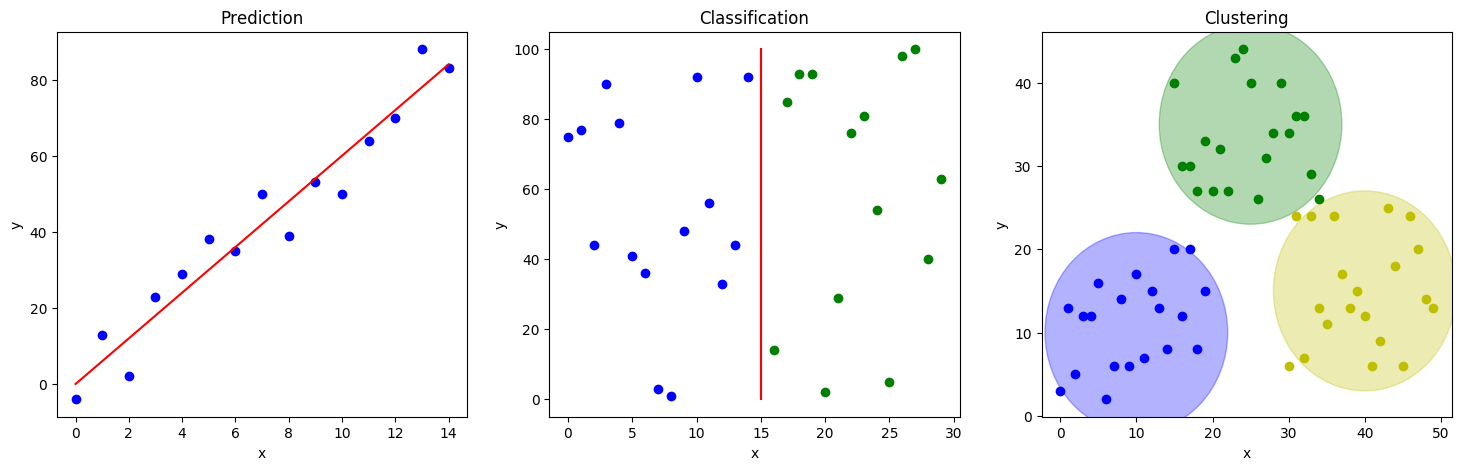
\includegraphics[width=\textwidth]{images/ml_problem_types.png}
	\caption{Arten von \textit{Machine Learning} Problemen (Quelle: Author)}
	\label{fig:ml_problem_types}
\end{figure}


\subsection{Ansätze}
\label{sec:ml_types}

Um ein ML-\textit{Model} anzulernen gibt es verschiedene Möglichkeiten. An eine davon - das Überwachte Lernen - wurde bereits in der Einführung anhand eines Beispiels herangeführt. Dieses Unterkapitel geht auch auf die anderen Möglichkeiten ein.

\subsubsection{Überwachtes Lernen}
Beim Überwachten Lernen (engl. \textit{supervised learning}) wird dem \textit{Model} ein Datenset bestehend aus Datenpunkten und den dazugehörigen korrekten Antwort zu einer Frage übergeben. Der ML-Algorithmus versucht aufgrund den Eigenschaften eines Datenpunktes einen Zusammenhand zu der Antwort zu finden. Wenn daraufhin neue Datenpunkte hinzugefügt werden, kann das \textit{Model} basierend auf den Eigenschaften eine Antwort prognostizieren. Das folgende abstrakte Beispiel demonstriert wie \textit{supervised learning} funktioniert.

Seit der Geburt lernt ein Kind, wie bestimmte Objekte aussehen und wie sie heißen. Es sieht jeden Tag einen Hund in verschiedenen Postionen, mal sitzend, laufend, stehend usw. Dadurch kann es auch den Nachbarshund als solchen identifizieren und zwischen einer Katze unterscheiden. Während der Lernphase kann natürlich auch ein Fehler vorkommen und zum Beispiel einen Wolf als einen Hund misinterpretieren. Doch die Eltern und Geschwister erklären dem Kind, dass es sich dabei nicht um einen Hund handelt. Es passt daher das Verständnis an und wird immer besser das Tier zu identifizieren. Im Kontext von ML ist die oben beschrieben Anwendung zur Erkennung von handgeschriebenen Buchstaben genauso überwachtes Lernen.

\subsubsection{Nicht-Überwachtes Lernen}
Bei dieser Art des Lernens sind im Datenset nicht die korrekten Antworten zu den einzelnen Datenpunkten enthalten. Der Algorithmus ist darauf ausgelegt Trends zu erkennen und Datenpunkte mit Gemeinsamkeiten zu gruppieren ohne zu wissen, worum was es sich dabei handelt. Um auf das oben beschrieben Beispiel mit dem Hund zurück zukommen, werden in einem \textit{Model} viele Bilder von verschiedenen Tieren eingespielt. Die Bilder sind jedoch nicht mit dem darauf enthaltenen Tier markiert. Nachdem der Algorithmus alle Charakteristiken der Bilder analysiert hat ist das \textit{Model} in der Lage, gleichartige Bilder zusammen zufassen. Es kann somit eine Gruppe erstellen, die alle Hunde enthält und eine andere, der alle Katzen zugeordnet sind. Am Ende hat das ML-\textit{Model} noch immer keine Vorstellung, um welches Tier es sich tatsächlich handelt.

Ein anderes Beispiel ist in der Analyse von Kaufverhalten zu finden. Das Datenset besteht hierbei aus den verschiedenen gekauften Produkten der Kunden und das Ziel ist Korrelationen darin zu finden. Das \textit{Model} soll in der Lage sein zum Beispiel folgendes bestimme zu können: Kunden die Schultaschen kaufen, kaufen auch Stifte. Oder Kunden die Bier kaufen, kaufen auch Chips.

\subsubsection{Teil-Überwachtes Lernen}
Teil-Überwachtes Lernen (engl. \textit{semi-supervised learning}) liegt zwischen den beiden vorher beschriebenen Arten des Lernens. Es wird ein Datenset verwendet, dass hauptsächlich aus unmarkierten Datenpunkten besteht. Ein kleiner Teil davon hat jedoch eine Markierung. Im ersten Schritt kommen Techniken zur Gruppierung zum Einsatz, um gleichartige Datenpunkte zu bündeln. Der zweite Schritt besteht darin, die bereits bekannten Datenpunkte dazu zu verwenden, andere Daten in der gleichen Gruppe zu markieren. Einer der größten Vorteile davon ist, dass nicht viel Zeit für das manuelle Markieren von Daten aufgewendet werden muss. Der Nachteil ist aber, dass es im vergleich zum Überwachten Lernen komplexer ist.

Auch hier lässt sich das Beispiel mit den Tieren anwenden. Aus Zeit- oder anderen technischen Gründen können nicht alle Bilder von Hunden und Katzen durchgesehen und markiert werden. Bei ein paar ist es jedoch möglich. Beim Teil-Überwachten Lernen gruppiert zuerst das ML-\textit{Model} alle Bilder mit Hunden und Katzen (gleiche Eigenschaften). Danach können aus den paar Markierten alle anderen abgeleitet werden.

\subsubsection{Bestärkendes Lernen}
Die letzte hier vorgestellte Art ist das Bestärkendes Lernen (engl. \textit{reinforcement learning}). Es kommt einerseits zum Einsatz, wenn sich die Situationen fortlaufend ändern, zum Beispiel beim Autofahren oder bei einem Spiel. Das \textit{Model} muss sich hierbei immer an neue Bedingungen anpassen. Andererseits wird es auch verwendet, wenn ein großer Zustandsraum existiert. Bei beispielsweise Schach ist es kaum möglich mittels \textit{brute-force} den besten nächsten Zug herauszufinden, da es viel zu viele Möglichkeiten im Verlauf eines Spieles gibt. Der Algorithmus ist also darauf ausgelegt eine Entscheidung basierend auf den momentanen internen Zustand und der Umgebung zu treffen, um ein vordefiniertes Ziel zu erreichen. Ein Ziel kann gegebenenfalls sein, ein Auto innerhalb der Spur zu halten. Je länger der Algorithmus lernen kann, desto besser und genauer werden die Entscheidungen in Hinblick auf eine langfristige Auswirkung.

\subsection{Regression}
\label{sec:ml_regression}

Die Regressionsanalyse (engl. \textit{regression analysis}) ist eine auf Statistik basierende \textit{Machine Learning}-Technik, welche aufgrund von oftmals historischen Daten zur Vorhersage verwendet wird. Dabei werden Relationen in markierten Daten analysiert, um eine Prognose für bestimmte Eigenschaften treffen zu können. Zum Beispiel kann damit ein \textit{Model} erstellt werden, welches den aktuellen Preis einer Immobilie bestimmt. Die historischen markierten Daten können hier die Eigenschaften Quadratmeteranzahl, Nachfrage, Lage als Kategorie, Kaufpreis, Verkaufspreis etc. haben. Im Kontext von ML werden die Eigenschaften als \textit{Features} bezeichnet

\section{CAN Bus}
\label{sec:can_bus}

Was ist der CAN Bus?

\subsection{DBC Datei}

was is a dbc datei

\subsection{MDF}

\textit{Measurement Data Format} (MDF) ist ein binäres Dateiformat, welches 1991 von der Firma Vector Informatik GmbH in Zusammenarbeit mit der Robert Bosch GmbH entwickelt wurde. Es ist speziell für Messdaten im Automotive-Bereich konzipiert und ist seit 2009 in der Version 4 als offizieller Standard von \textit{Association for Standardization of Automation and Measuring Systems} (ASAM) öffentlich zugänglich. Ein wesentlicher Vorteil des Formates ist, dass die Messdaten sehr schnell und speicherplatzsparend abgespeichert werden können. Des Weiteren wird auch eine Optimierung des Lesevorgangs durch Vorsortierung und Indizierung unterstützt. Neben den eigentlichen Nutzdaten werden auch Metadaten aus der DBC-Datei mitgespeichert. Dies ist vor allem für weitere Analysen und die Interpretierung der Rohdaten notwendig. Beispielsweise gehören die Information zur Umwandlung in physikalische Werte und Signalnamen dazu. \cite{ASAM14}

\section{Embedded Devices}
\label{sec:embedded_devices}

Vielleicht auch Einführung in Embedded Systems?


% \begin{figure}[htbp]
% 	\centering
% 		
\includegraphics{images/birne}
% 	\caption{Eine Glühbirne}
% 	\label{fig:birne}
% \end{figure}



% \section{Unterkapitel 21}
% \label{sec:Unterkapitel21}

% Textkörper mit Tabelle.

% \begin{table*}[htbp]
% 	\centering
% 		\begin{tabular}{|l|c|r|}
% 		\hline
% 		\rowcolor[gray]{0.9}
% 		Spalte 1 & Spalte 2 & Spalte 3 \\
% 		\hline
% 		Affen & Giraffen & Löwen \\
% 		äpfel & Birnen & Bananen \\
% 		Irgend & et & was \\
% 		\hline
% 		\end{tabular}
% 	\caption{Beispiel für eine Tabelle}
% 	\label{tab:BeispielFuerEineTabelle}
% \end{table*}

% Man beachte die Gegenüberstellung in Tabelle \ref{tab:BeispielFuerEineTabelle}.

% \section{Unterkapitel 23}
% \label{sec:Unterkapite23}

% Aufzählungen:

% Nummeriert:

% \begin{enumerate}
% 	\item Punkt 1
% 	\item Punkt 2
% \end{enumerate}

% Mit Bullet Points:

% \begin{itemize}
% 	\item Punkt 1
% 	\item Punkt 2
% \end{itemize}

% Mit Beschreibungen:

% \begin{description}
% 	\item[Item 1] das ist der 1.Punkt
% 	\item[Item 2] und das der 2.
% \end{description}


% Auch Programmcodes können an entsprechender Stelle eingefügt werden, man beachte dazu auch Listing \ref{lst:conv}.

% % see also http://mirror.easyname.at/ctan/macros/latex/contrib/listings/listings.pdf for options

% \begin{lstlisting}[frame=lines, caption=Simple Listing, captionpos=b, label = lst:conv, language=C, showstringspaces=false]
% #include <stdio.h>
% int main()
% {
% 	int i, n, t1 = 0, t2 = 1, nextTerm;

% 	printf("Enter the number of terms: ");
% 	scanf("%d", &n);

% 	printf("Fibonacci Series: ");

% 	for (i = 1; i <= n; ++i)
% 	{
% 		printf("%d, ", t1);
% 		nextTerm = t1 + t2;
% 		t1 = t2;
% 		t2 = nextTerm;
% 	}
% 	return 0;
% }
% \end{lstlisting}

% Und zuguterletzt, Formeln mitten im Fliesstext, wie z.B. $a^2+b^2=c^2$, in einem Absatz.


%----------------------------------------------------------------
%
%  File    :  implementation.tex
%
%  Authors :  David Lechner, FH Campus Wien, Austria
%
%  Created :  10 Oct 2019
%
%  Changed :  10 Oct 2019
%
%----------------------------------------------------------------


\chapter{Umsetzung}
\label{chap:back}

Dieses Kapitel geht auf die konkrete Umsetzung des Systems ein. Anfangs werden die zur Verfügung stehenden Daten beschrieben und wie diese für \textit{Machine Learning} vorverarbeitet werden. Danach werden die eingesetzten ML-\textit{Model} erklärt und die Optimierung dieser gezeigt. Den Abschluss bildet die Integration in ein Fahrzeug.

\section{CAN-Daten}
\label{sec:data_description}

Bei den Daten, welche für die Masterarbeit vorliegen, handelt es sich um CAN-Nachrichten, aufgenommen in zehn Fahrzeugen (VW Golf 7, keine näheren Informationen) während dem Fahren. Dabei ist sichergestellt, dass jeweils nur eine Person hinter dem Lenkrad gesessen ist. Für die Aufzeichnung wurde ein Boardcomputer mit Internetkonnektivität (\textit{ALEN}, siehe \ref{sec:alen}) im Fahrerraum verwendet. Das \textit{Embedded-Device} ist über zwei CAN-Bus Schnittstellen mit der Fahrwerks-Linie (F-CAN) und der Fahrzeugelektrik-Linie (K-CAN) verbunden und kann somit alle Nachrichten in fast-echtzeit vom Bus mitlesen. Dabei ist aber sichergestellt, dass es nicht möglich ist, auch Nachrichten senden zu können, da dies bei einer Fehlfunktion zu einem Unfall führen und Insaßen gefährden könnte. Die Nachrichten werden nach dem Empfangen mit einem synchronisierten Zeitstempel, aufgelöst in Nanosekunden, versehen und in eine MDF Datei mit den Metadaten von der entsprechenden DBC-Datenbank gespeichert. Eine Datei enthält jeweils Messdaten über eine Dauer von einer Minute. Danach wurde die Datei temporär auf einer Festplatte gespeichert und auf einem File-Server über eine LTE-Funkverbindung hochgeladen. Um sie über alle Fahrzeuge hinweg eindeutig zuordnen zu können, wurde eine Fahrzeugidentifikationsnummer dem Dateinamen angehängt.

In einer Datei sind 46 verschiedene Signale der beiden CAN-Busse enthalten. Tablle \ref{tab:can_signals} listet die meisten davon. Jene, die sich vorrausichtlich nicht für die Analyse eignen, wie z.B. die innen Temperatur oder der Status des Standlichts, sind ausgenommen. Für die komplette Liste siehe Anhang. Pro Datei sind durchschnittlich 100000 Messwerte vorhanden, daraus ergeben sich bei einer Anzahl von 10359 Dateien über eine Milliarde Messpunkte. Die folgende Liste gibt einen Einblick über die vorhandenen Daten.
% TODO: Anhang mit kompletter Liste

\begin{itemize}
  \item Anzahl Fahrer: 10
  \item Datengröße (MDF): 3,7 GB
  \item $\diameter$ Fahrtenanzahl: 1
  \item Fahrtenanzahl insgesamt: 7
  \item $\diameter$ Fahrtzeit pro Fahrer pro Fahrt: 13
  \item $\diameter$ Fahrtzeit pro Fahrer: 14
  \item Fahrtzeit insgesamt: 87
  \item $\diameter$ Gefahrene Kilometer: 14
  \item Gefahrene Kilometer insgesamt: 84
  \item Zeitraum: 12.09.2019 - 13.08.2019
\end{itemize}

\begin{table*}[htbp]
	\centering
		\begin{tabular}{|l|l|l|l|l|}
		\hline
		\rowcolor[gray]{0.9}
		Signalname & CAN-Bus & Beschreibung & Einheit & Wertbeschr. \\
		\hline
    LWI\_Lenkradwinkel & F-CAN & Lenkradwinkel & Grad & - \\
    LWI\_VZ\_Lenkradwindel & F-CAN & \shortstack{Vorzeichen von \\ Lenkradwinkel} & Boolean & \shortstack{0: Positiv \\ 1: Negativ} \\
    ESP\_Fahrer\_bremst & F-CAN & Bremspedal betätigt & Boolean & \shortstack{0: nicht betätigt \\ 1: betätigt} \\
    ESP\_Bremsdruck & F-CAN & Bremsdruck & Bar & - \\
    MO\_Fahrpedalrohwert\_01 & F-CAN & Fahrpedalposition & - & - \\
    MO\_Kuppl\_schalter & F-CAN & Kupplung betätigt & Boolean & \shortstack{0: nicht betätigt \\ 1: betätigt} \\
    MO\_Drehzahl\_01 & F-CAN & Motordrehzahl & rpm & - \\
    KBI\_Tankfuellstand\_Prozent & F-CAN & Tankfüllstand & \% & - \\
    KBI\_Kilometerstand & F-CAN & Kilometerstand & km & - \\
    MO\_Gangposition & F-CAN & Gangposition & - & \shortstack{1: 1. Gang oder \\ Rückwärtsgang \\ 2-6: 2. - 6. Gang} \\
    ESP\_VL\_Radgeschw\_02 & F-CAN & \shortstack{Geschwindigkeit \\ Rad links vorne} & km/h & - \\
    ESP\_VR\_Radgeschw\_02 & F-CAN & \shortstack{Geschwindigkeit \\ Rad rechts vornen} & km/h & - \\
    ESP\_HL\_Radgeschw\_02 & F-CAN & \shortstack{Geschwindigkeit \\ Rad links hinten} & km/h & - \\
    ESP\_HR\_Radgeschw\_02 & F-CAN & \shortstack{Geschwindigkeit \\ Rad rechts hinten} & km/h & - \\
    ESP\_v\_Signal & F-CAN & \shortstack{Durchschnittliche \\ Radgeschwindigkeit} & km/h & - \\
    ESP\_HL\_Fahrtrichtung & F-CAN & \shortstack{Fahrtrichtung \\ Rad links hinten} & - & \multirow{2}{*}{\shortstack{0: Vorwärts \\ 1: Rückwärts}} \\
    ESP\_HL\_Fahrtrichtung & F-CAN & \shortstack{Fahrtrichtung \\ Rad links hinten} & - & \\
    ESP\_Laengsbeschl & F-CAN & Längsbeschleunigung & m/s\textsuperscript{2} & - \\
    ESP\_Querbeschleinigung & F-CAN & Querbeschleunigung & m/s\textsuperscript{2} & - \\
    ESP\_Gierrate & F-CAN & Gierrate & \shortstack{Grad pro \\ Sekunde} & - \\
    ESP\_VZ\_Gierrate & F-CAN & \shortstack{Vorzeichen \\ von Gierrate} & Boolean & \shortstack{0: Positiv \\ 1: Negativ} \\
    Wischer\_vorne\_aktiv & K-CAN & Wischer vorne aktiv & Boolean & \multirow{3}{*}{\shortstack{0: nicht aktiv \\ 1: aktiv}} \\
    BH\_Blinker\_li & K-CAN & Blinker links aktiv & Boolean & \\
    BH\_Blinker\_re & K-CAN & Blinker rechts aktiv & Boolean & \\
		\hline
		\end{tabular}
	\caption{Signalbeschreibung}
	\label{tab:can_signals}
\end{table*}

Je nach Steuergerät und Nachrichtentyp ist die Signalhäufigkeit unterschiedlich. Zum Beispiel sendet das Lenkrad- und Motorsteuergerät mit der gleichen Frequenz – nämlich 100-mal in der Sekunde. Andere jedoch, wie das Getriebesteuergerät, nur mit einer Frequenz von 10 Hz. Abbildung \ref{fig:signal_freq} zeigt Häufigkeit einiger Signale.

\begin{figure}[htbp]
	\centering
		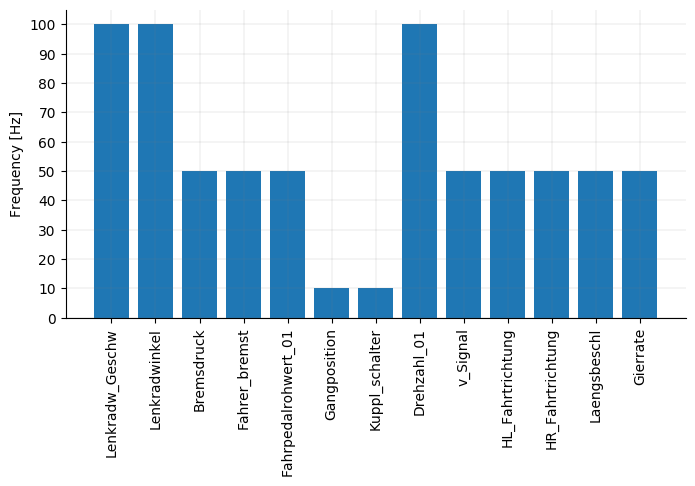
\includegraphics[width=\textwidth]{images/signal_frequences.png}
	\caption{Signalhäufigkeiten (Quelle: Author)}
	\label{fig:signal_freq}
\end{figure}

\section{Trainingsdaten}
\label{sec:train_data}

Relevante

Data transformation

Feature extraction

\section{Machine Learning Model}
\label{sec:ml_implementation}

Wieso supervised und nicht zb unsupervised? daten sind bereits markiert, kein zeitaufwand notwendig, bessere genauigkeit. trotzdem probieren! ML Model beschreiben, Code snippets

\subsection{Optimierung}
\label{sec:ml_optimization}

Hyper parametering, trade of performance - accuracy

\section{Integration in Auto}
\label{sec:car_integration}

ML auf ALEN Box

\subsection{Automotive Linux Edge Node (ALEN)}
\label{sec:alen}

%----------------------------------------------------------------
%
%  File    :  discussion.tex
%
%  Authors :  David Lechner, FH Campus Wien, Austria
%
%  Created :  10 Oct 2019
%
%  Changed :  10 Oct 2019
%
%----------------------------------------------------------------


\chapter{Diskussion}
\label{chap:discussion}

Das letzte Kapitel vor der Zusammenfassung präsentiert die erzielten Ergebnisse der Masterarbeit und diskutiert die Erkenntnisse. Die Gliederung spiegelt die behandelten Forschungsfragen. Des Weiteren wird ein Ausblick über weiterführende Tätigkeiten gegeben.

\section{Validierung der Methoden}

Im Abschnitt \ref{sec:related_work} wurden vier Paper vorgestellt, welche sich mit dem gleichen Thema - Fahreridentifikation basierend am Fahrverhalten - beschäftigen. Diese haben hauptsächlich den \textit{Machine Learning} Algorithmus \textit{Random Forest} verwendet und damit gute Resultate erzielen können (teilweise über 85\%). Es wurde jedoch sehr wenig über die Struktur, Eigenschaften und Herkunft der Daten erwähnt. Daher war die erste Frage: Sind die existierenden Methoden mit den vorhandenen Daten valide? Kapitel \ref{chap:set_up} hat gezeigt, dass dies zutrifft, da bei einem ersten Versuch eine Genauigkeit des Modells von 85\% herausgekommen ist. Weitere Durchläufe haben hingegen eine hohe Schwankungsbreite - von 78,66\% bis 92,53\% - ergeben. Das lässt sich auf zwei Gründe zurückführen. In Sektion \ref{sec:feature_optimization} bei der \textit{Feature}-Analyse wurde entdeckt, dass das Signal \textit{Gangposition} Unregelmäßigkeiten aufweist. Bei fünf von neun Datensets ist der Wert durchgehend \textit{14}. Die guten Ergebnisse (über 90\%) können zum Teil daher kommen, dass das Trainings- und Testset gleichverteilt Datenpunkte mit und ohne Gangposition \textit{14} haben. Dadurch bekommt, wie in Abbildung \ref{fig:feature_importance} gezeigt, das \textit{Feature} eine große Bedeutung und hilft ungemein bei der Klassifizierung. Der zweite Grund ist, dass die Auswahl der Daten einen Einfluss auf die Genauigkeit haben. Befinden sich viele Autobahnkilometer, welche wenig Individualität aufweisen und schwerer zuordenbar sind, unter den Sets, sinkt die Trefferquote. Das Gegenteil tritt bei vielen Datenpunkten von Lenk- oder Bremsmanöver auf, die Trefferquote steigt.

Das \ref{chap:set_up}. Kapitel hat die vorliegenden Daten beschrieben. Im Gegensatz zu \cite{Gahr2018} sind sie direkt von mehreren CAN-Linien abgegriffen worden und nicht über den Diagnostik-Port (OBD II). Das bringt einige Vorteile. Zum Beispiel sind aufgrund dessen alle vorhandenen Signale am Bus verfügbar. Alleine am Fahrwerks-CAN sind bis zu 1500 und am Komfort-CAN über 2500 Signale vorhanden. Je nach Hardwarekapazitäten und Fahrzeugmodell können auch noch mehrere CAN-Linien miteinbezogen werden. Damit wird das ML-Modell genauer und aussagekräftiger, wenn es mehr Daten zum Verarbeiten gibt. Währenddessen über den OBD II Port \cite{SAEII} laut Spezifikation maximal 196 Signale übertragen werden. Hier handelt es sich meist auch nur um verschiedenen Abgaswerte, Fehlerhistorie und Temperaturen. Hersteller können zudem noch weitere Signale in die Schnittstelle implementieren, welche aber nicht spezifiziert sind. Um die Werte über OBD II auslesen zu können, muss ein Dongle eingesetzt werden, der in einen dezidierten Anschluss, meist versetzt unterhalb des Lenkrads, eingesteckt wird. Er hat das OBD Protokoll implementiert und kann die Signale auswerten und in die physikalische Einheit umrechnen \cite{OBD20}. Für die Weiterverarbeitung wird gewöhnlich eine Bluetooth-Verbindung zu einem weiteren Gerät (z.B. Smartphone) benötigt. Für diese Anwendung wäre die ALEN notwendig, die die Daten empfängt und mit dem \textit{Machine Learning} Algorithmus klassifiziert. Durch den OBD II Dongle ergeben sich zusätzlich einige Angriffsvektoren, mithilfe dieser die Privatsphäre verletzt, Eigentum beschädigt und sogar Leib und Leben gefährdet werden könnte. Forscher haben hierzu 77 am Markt verfügbare Dongles getestet und sind zum Entschluss gekommen, dass alle mindestens zwei Schwachstellen enthalten \cite{USENIX20}. Beispielsweise sind keine Authentifizierungsmethoden realisiert, lassen das Extrahieren der Firmware ohne Sicherheitsmechanismus zu oder senden CAN-Nachrichten am Bus ohne jegliche Validierung. Das Abgreifen direkt vom Bus ist daher die klar bessere Methode und bietet mehr Signale, bessere Sicherheit und Schutz der Privatsphäre.

\section{Optimierung}

Bei der Beantwortung der zweiten Forschungsfrage wurde versucht, den \textit{Random Forest} Algorithmus zu optimieren. Im ersten Schritt sind die Parameter analysiert worden. Dabei hat sich herausgestellt, dass die Standardwerte bereits sehr gute Ergebnisse liefern. Selbst nach 16128 Durchläufen, bei denen jede mögliche Kombination der Parameter überprüft wurde, konnte lediglich eine Verbesserung um fast ein Prozent erzielt werden. Auffallend war, dass eine Veränderung des Wertes bei dem Parameter \textit{criterion} - von \textit{gini} auf \textit{entropy} - zwar keine Auswirkung auf die Trefferquote gehabt hat, jedoch sich die Durchlaufzeit erheblich vergrößert hat, nämlich um mehr als 300\%. Der Grund hierfür ist die dahinterstehende Formel. \textit{Entropy} wird mit dem Logarithmus der Basis 2 von der Wahrscheinlichkeit berechnet, wohingegen bei der \textit{Gini Impurity} die Wahrscheinlichkeit mit sich selbst multipliziert wird (siehe \ref{sec:random_forest}). Da die Logarithmus-Funktion mehr Rechenleistung erfordert als eine Multiplikation, ist das Aufteilen eines Knotens mit \textit{entropy} langsamer.

Durch eine detailliertere Analyse der vorhanden Datensätze hat sich eines verdeutlicht: Die Daten sind das ausschlaggebendste für die \textit{Machine Learning} Anwendung. Diese Aussage wird auch immer wieder in der Literatur (\cite{Rebala2019}, \cite{Conway2012}) bestätigt. Damit ist gemeint, dass zum einen die Struktur einheitlich und bekannt und zum anderen ausreichend viele Daten erhältlich sein müssen. Gibt es beispielsweise mehrere fehlende Werte oder Unregelmäßigkeiten (siehe \textit{Gangposition}) können manche ML Algorithmen nicht zuverlässig Ergebnisse liefern. Das gleiche gilt wenn einfach zu wenig verfügbar sind. Das Regelset des Modells kann so nicht hinreichend gebildet werden, um die Vielfalt der existierenden Daten abzubilden.

Ein ML-\textit{Model} stellt in gewisser Weise eine \textit{Blackbox} dar, da nicht ohne einer näheren Untersuchung erkennbar ist, auf Grund welcher Daten eine Entscheidung getroffen wird. Diese Erfahrung hat auch der Autor von \cite{Gahr2019} gemacht, der ebenfalls den Lenker anhand von CAN- und Smartphone-Daten identifizieren wollte. Er hat das Modell mit allen zugänglichen Daten trainiert, darunter auch Längen- und Breitengrade des GPS-Moduls. Der \textit{Classifier} hat am Ende nicht basierend am Fahrverhalten Datenpunkte zugeordnet, sondern alleine mittels den GPS-Daten. In Abschnitt \ref{sec:feature_importance} wurde ähnliches aufgezeigt. Mit Hilfe der integrierten \textit{Feature Importance} des \textit{Random Forest}s ist bemerkt worden, dass es beim Signal \textit{Gangposition} keine durchgängigen Werte gibt. Der Missstand wurde bereits oben erläutert und bekräftigt die genannte These, dass die Daten vor dem Einsatz mit \textit{Machine Learning} genauestens analysiert und validiert werden müssen. Das verhindert eine falsche Vorgehensweise des ML-Modells als \textit{Blackbox}.

\section{Dauer der Trainings- und Identifikationsphase}

Im Zuge der Optimierungen und der Integration wurde auch die Fragestellung behandelt, wie viele Trainingsdaten vonnöten sind, um mindestens 85\% Genauigkeit des \textit{Models} zu erreichen. Des Weiteren war die Frage, wie lang eine Person fahren muss, damit sie zu 85\% identifiziert werden kann. Hier kann keine pauschale Antwort gegeben werden, da viele Faktoren Einfluss darauf nehmen. Mitsicherheit die maßgeblichsten davon sind die Anzahl an Fahrprofilen in einem Set und welche Daten ausgewählt werden. Die Abbildungen \ref{fig:train_duration_shuffle} und \ref{fig:train_duration_start} zeigen den Unterschied zwischen einer zufälligen und chronologischen Auswahl. Bei ersteren ist die maximale Genauigkeit mit 40 Minuten Trainingszeit pro Fahrer bei etwa 75\% gelegen. Sind die Daten jeweils nach Fahrtbeginn für die Trainingsphase herangezogen worden, wurde nach ca. 15 Minuten knapp 86\% erreicht. Mit der Zufallsauswahl konnte das Ziel somit nicht erreicht werden. Das bestätigt die Annahme, dass Daten am Beginn einer Fahrt, wo mehrere Lenk- und Bremsmanöver stattfinden, eine höhere Individualität aufweisen und dadurch besser zu klassifizieren sind. Die beschriebenen Tests sind mit neun Fahrprofilen durchgeführt worden. Während der Integration hat ein Test mit nur vier eine Genauigkeit von 94\% ergeben. Das beweist, dass allein die Reduktion auf eine geringere Anzahl einen großen Einfluss hat.

Für die Dauer der Identifikationsphase gilt ebenso das gleiche. Da sich das Kapitel \textit{Optimierung} an erster Stelle auf die allgemeine Verbesserung des Modells konzentriert hat, ist dieser Aspekt nicht beleuchtet worden. Es liegen daher keine Ergebnisse für ein Modell mit neun Profilen vor. Das vorherige Kapitel ist jedoch explizit auf die Fragestellung eingegangen. Allerdings kann wieder keine pauschale Aussage getroffen werden, da ein paar Gegebenheiten vorausgesetzt waren. Zum einen sind im ML-Modell nur vier Datensätze inkludiert und zum anderen gibt es eine Einschränkung durch die Zeit die benötigt wird, um den \textit{Random Forest Classifier} zu trainieren. Des Weiteren ist die Art der Identifizierung durch den eingesetzten Algorithmus (siehe \ref{sec:identification_difference}) gesteuert. So muss zum Beispiel fünfmal ($\widehat{=}$ 5 Minuten) hintereinander die gleiche Fahrerin identifiziert werden. Mehreren Tests mit verschiedenen Daten haben hierbei ergeben, dass 97\% davon im Durchschnitt nach 5,73 Minuten identifiziert sind.

\section{Integration}

Die letzte Forschungsfrage zielt auf die Integration des Systems zur Fahreridentifikation in ein Fahrzeug ab. Wie in dem Kapitel beschrieben, ist es nicht möglich gewesen, da ein tatsächliches Auto nicht zur Verfügung gestellt wurde. Stattdessen ist der CAN-Bus durch die bereits vorhandenen Daten simuliert worden. Die Beschreibungen und Ergebnisse haben gezeigt, dass dies sehr gut funktioniert hat und es auf diese Weise zu fast realen Bedingungen gekommen ist. Die ALEN als zentrale Einheit eignet sich prinzipiell gut für diesen Einsatz, da sie die notwendige Peripherie mitbringt, hat aber klar ihre Grenzen in Bezug auf \textit{Machine Learning}. So dauert es ca. fünf Minuten, bis die CCU den \textit{Random Forest Classifier} erstellt und trainiert hat. Einige Maßnahmen könnten die Zeit reduzieren. Beispielsweise kann die ALEN durch eine leistungsstärkere CCU mit sonst ähnlicher Hardwareausstattung ersetzt werden. Denkbar wäre zudem, das trainierte Modell zu speichern und bei Fahrtbeginn nur zu laden. Den Prozess komplett in die \textit{Cloud} auszulagern, erfordert das Umsetzen von weitgehenden \textit{Security}- und \textit{Privacy}-Anforderungen, da sich die persönlichen Fahrprofile nicht mehr nur lokal im Auto befinden. Weiters würde dadurch das Konzept von \textit{Edge Computing} verloren gehen. Die Vorteile davon wurden in den Grundlagen näher gebracht, hat aber eben auch einen Nachteil, nämlich der von fehlenden Ressourcen am \textit{Edge Device}, vorausgesehen.

Selbst wenn die Zeit auf ein Minimum reduziert werden könnte, würde es die Identifizierung nicht zwangsläufig beschleunigen. Sie hängt hauptsächlich vom Zweck ab und wird von der Konfiguration des \textit{ML-Model Predictor} bestimmt. Dem Serviceanbieter - sei es der OEM oder eine Drittpartei - muss klar sein, dass je kürzer die Identifikationsphase gewählt wird, desto leichter kann es zu einer Missidentifikation kommen. Es gibt durchaus Services, welche erst gegen Ende einer Fahrt die Identifikation benötigen. Zum Beispiel ist in der Einleitung das digitale Fahrtbuch besprochen worden, das vollkommen ohne jeglicher Interaktion seitens der Fahrerin auskommt. Eine Implementierung auf der ALEN wäre ohne viel Zutun möglich, da dort bereits alle Daten aufliegen. Eine weitere Einsatzmöglichkeit liegt bei \textit{Car-Sharing} Anbietern. Sie können mit Hilfe des Systems erkennen, ob wirklich die registrierte Person hinter dem Lenkrad sitzt. Diese Information genügt es auch erst am Ende zu haben. Das gleiche Prinzip lässt sich zudem bei Mietwagenunternehmen realisieren. Die Standardverträge erlauben nur einen Lenker, jede weitere kostet extra Geld (\EUR{8,50} bei \textit{Sixt} \cite{SIXT}). Die Überprüfung kann hiermit durchgeführt und bei Bedarf der Vertragszusatz automatisiert ergänzt werden.

Es gibt überdies Anwendungen, die eine schnelle Identifikation erfordern. Eine davon, die Diebstahlwarnung, wurde ebenfalls schon in der Einleitung erwähnt und in diesen Kontext gesetzt. Für die Umsetzung wäre bloß eine kleine Adaption der vorhandenen Anwendung notwendig, bei der eine zusätzliche Abfrage zu unzureichenden Klassifizierungen eingebaut wird. Nachdem mehrere Versuche Dateien korrekt zuzuordnen gescheitert sind, kann eine SMS an den Fahrzeughalter gesendet werden, die darüber informiert, dass womöglich eine nicht autorisierte Person das Fahrzeug steuert. Hier muss aber klar geprüft werden, ab wann entschieden wird, dass es sich wirklich um einen unbekannten Fahrer handelt und nicht um einen bekannten, der noch nicht identifiziert wurde.

Durch die Ergebnisse des letzten Kapitels ist davon auszugehen, dass ein paar Minuten an Fahrzeit benötigt werden, damit eine Lenkerin ausreichend erkannt wird. Aus diesem Grund sind einige Services nicht umsetzbar. Allen voran jene, welche unmittelbar nach Fahrtbeginn in Kraft treten würden. Das automatische Einstellen des bevorzugten Radiosenders oder das Einrichten der Außenspiegel fallen somit weg. Ebenso die Möglichkeit, dass Fahrerabhängig bestimmte \textit{Features} de- und aktiviert werden, ist nicht vorstellbar. Das gleiche gilt für eine Drosselung der Leistung, wenn beispielsweise noch unerfahrene Personen hinter dem Steuer sitzen. Dies könnte gegebenenfalls sogar eine Gefahr darstellen, da in der Anfangszeit die volle Leistung zu einem erhöhten Unfallrisiko beiträgt.

\section{Limitierungen}

Da nur eine geringe Anzahl an Fahrdaten vorliegen, kann keine Aussage über die Genauigkeit des Systems in einer diverseren Umgebung erfolgen. Zudem fehlen CAN-Nachrichten von mehr Fahrzeugtypen, um das Modell mit den Signalen validieren zu können. Des Weiteren sind keine Informationen über Geschlecht, Altersgruppen und Dauer des Führerscheinbesitzes von den vorhandenen Fahrprofilen bekannt. Es ist daher auch unklar, ob es sich dabei um eine repräsentative Gruppe an Testpersonen handelt. Bei nur neun ist es anzunehmen. Obwohl die Simulation den realen Bedingungen sehr nahe kommt, können trotzdem nicht alle Eventualitäten abgebildet werden. Das resultiert wahrscheinlich in einer Abweichung der Zuverlässigkeit der Anwendung.

\section{Ausblick}

Um das vorgestellte System zur Fahreridentifikation zu verbessern, gibt es mehrere Möglichkeiten. Neben dem \textit{Random Forest} sind in der Literatur auch andere Algorithmen zur Klassifizierung (\cite{Rebala2019}, \cite{Enev2016}) beschrieben. Bei einem Vergleich könnte sich ein anderer als performanter und genauer herausstellen. Das Modell kann zusätzlich optimiert werden, indem eine \textit{Feedback}-Schleife implementiert wird. Nach einer erfolgreichen Identifikation werden die neuen Messpunkte dem Modell als neue Trainingsdaten zur Verfügung gestellt. Dadurch lernt der \textit{Classifier} durchgehend neue Fahrsituationen. Ein anderer Ansatz wäre nur Datenpunkte herzunehmen, welche leichter zu klassifizieren sind. Kapitel \ref{chap:set_up} und \ref{chap:optimization} haben aufgezeigt, dass solche existieren. Hier stellt sich die Frage, welche Fahrmanöver eine höhere Individualität aufweisen. Die Messdateien können folglich im \textit{Data-Preprocessor} auf die relevanten Daten reduziert werden. Als Anhaltspunkt dienen hierfür die Arbeiten \cite{Gahr2018} und \cite{Hallac2016}, die sich zum Teil schon damit beschäftigt haben.

Ein weiterer Punkt ist die Anwendung mit einem echten Fahrzeug zu erproben, da dies nicht möglich war. Im Zuge dessen ist eine Überprüfung der Simulationsergebnisse möglich. Außerdem wäre es interessant zu wissen, ob sich das System durch eine manipulierte Fahrweise austricksen lässt. Dadurch kann die Stabilität getestet werden und ob die Fahrweise von einer Person nachgeahmt werden kann.

%----------------------------------------------------------------
%
%  File    :  conclusion.tex
%
%  Authors :  David Lechner, FH Campus Wien, Austria
% 
%  Created :  10 Oct 2019
% 
%  Changed :  10 Oct 2019
% 
%----------------------------------------------------------------


\chapter{Zusammenfassung}
\label{chap:conclusion}

Zusammenfassung



%% ....


% --- Verzeichnisse ------------------------------------------------------

\newpage
%\chapter{Verzeichnisse}

% --- Bibliography ------------------------------------------------------

\bibliographystyle{alpha}

% List references I definitely want in the bibliography,
% regardless of whether or not I cite them in the thesis.

\newpage
%\phantomsection
%\addcontentsline{toc}{chapter}{Literaturverzeichnis}
\addcontentsline{toc}{chapter}{Bibliography}
\bibliography{thesis}

\newpage

% --- List of Figures ----------------------------------------------------

%\newpage
%\phantomsection
%\addcontentsline{toc}{chapter}{Abbildungsverzeichnis}
\addcontentsline{toc}{chapter}{List of Figures}
\listoffigures


% --- List of Tables -----------------------------------------------------

\newpage
%\phantomsection
%\addcontentsline{toc}{chapter}{Tabellenverzeichnis}
\addcontentsline{toc}{chapter}{List of Tables}
\listoftables

% --- List of Listings -----------------------------------------------------

\newpage
%\phantomsection
\addcontentsline{toc}{chapter}{Listings}
%\lstlistoflistings

          % List of figures/tables/listings; bibliography

\appendix
%----------------------------------------------------------------
%
%  File    :  appendix.tex
%
%  Authors :  David Lechner, FH Campus Wien, Austria
% 
%  Created :  10 Oct 2019
% 
%  Changed :  10 Oct 2019
% 
%----------------------------------------------------------------

\chapter{Anhang/Ergänzende Information}
\label{chap:app}

EIGENER ANHANG

(Hier können Schaltpläne, Programme usw. eingefügt werden.)

\clearpage		   % other appendices

\end{document}
